\section{Techniques Comparison}
\label{section:techniques}
Here is the comparison of the 3D-sensing techniques between autonomous navigation and the metaverse:
\\\\
\textbf{1.	Autonomous Navigation}
\\\\
The 3D-sensing techniques of Autonomous navigation is composed with \textbf{cameras, Radar, Ultrasound, IMU, and LiDAR sensors} surrounded around the car to simulate the actual environment beside the car.
\begin{figure}[H]
    \centering
    \subfigure{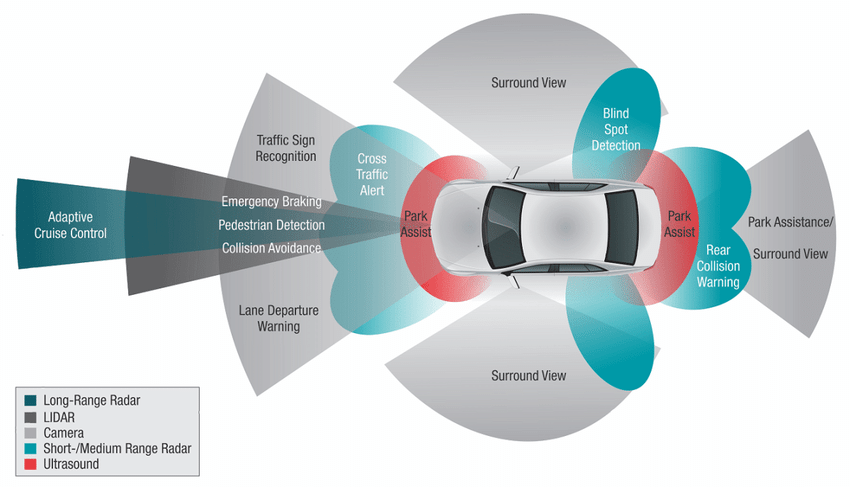
\includegraphics[width=.9\columnwidth]{images/Camera.png}}
    \caption[Short text]{3D-sensors in autonomous navigation \cite{autonomousPic}}
    \label{fig:Camera}
\end{figure}

(1)	\textbf{Camera} \cite{autonomousSensor}: To obtain 3D-colored images, at least two cameras are required.
\\\\
(2)	\textbf{Radar} \cite{autonomousSensor}: In recent decades they have also been installed in vehicles to measure distances to obtain reliable data for systems such as the spacer and the emergency brake assistant, regardless of weather conditions. The sensors emit short pulses in the form of electromagnetic waves (radio waves), which are propagated almost at the speed of light. As soon as the waves hit an object, they are reflected and bounce back to the sensor. The shorter the time interval between transmission and reception, the closer the object is. This technology enables the use of driver assistance systems such as adaptive cruise control and collision avoidance.
\\\\
(3)	\textbf{Ultrasound} \cite{autonomousSensor}: Ultrasound is used for the closed range danger detection (limited to less than 10 meters); it can detect the full surrounding of a car within a short-range. Ultrasound is mainly used for parking aid, monitoring the blind spot, and for emergency brake assistants. It is based on the time-of-flight principle, which emitted sound waves at a frequency of 20,000 Hz.
\\\\
(4)	\textbf{IMU} \cite{ARIMU} \cite{autonomousIMU}: The IMU provides information on current vehicle location and orientation. An IMU combines three types of sensors: an accelerometer, a gyroscope, and a magnetometer. The accelerometer measures linear acceleration, the gyroscope measures rotational acceleration, and the magnetometer is a device capable of measuring magnetism, which can help us find orientation using the earth's magnetic field, like a compass. Each of these sensing elements must also sense the measured property in 3 axes, (X, Y, Z). Each sensor employs a fabrication technology known as “MEMS”, Micro-Electro-Mechanical Systems. This fabrication technology is based on Integrated Circuit Photolithography techniques.
\\\\
(5)	\textbf{LiDAR} \cite{autonomousSensor}: In contrast to ultrasonic sensors, LiDAR sensors are suitable for both short- and long-range use. Although they have existed for many years, they have only been used increasingly in vehicles since the 2000s. LiDAR is considered a key technology for achieving higher levels of autonomy because they measure the distance of objects at incredible speeds and with high precision. LiDAR sensors emit up to one million laser pulses per second and summarize the results in a high-resolution 3D map of the environment.
\\\\
\textbf{2.	Metaverse}
\\\\
Metaverse combines the techniques of \textbf{Virtual Reality (VR), Augmented Reality (AR)}, and \textbf{the Internet}. As for AR \cite{metaverseSensor}, to augment our reality, the system must first understand exactly what reality it is they are working with. That is, both \textbf{camera} and \textbf{LiDAR} will be the best tool to quantify the spaces in our lives. \cite{ARIMU} Moreover, for a VR headset system to accurately adjust the projected image on the viewscreen, or an AR system to place the projected holographs, the computer must know the relative location and motion of the wearer’s head. An \textbf{Inertial Measurement Unit (IMU)} is typically used to accomplish this task.
\\\\
(1)	\textbf{Camera and LiDAR}: Used for environment simulation. Also used in the 3D-sensing of autonomous navigation.
\\\\
(2)	\textbf{Inertial Measurement Unit (IMU)}: Combining these signals facilitates error correction and yields accurate measurements to track head position and movement. Also used in the 3D-sensing of autonomous navigation.
\\\\
\textbf{In conclusion}, Metaverse uses Camera, LiDAR, and IMU to keep track of the user’s information as well as to simulate the environment. Similarly, autonomous navigation also takes advantage of Camera, LiDAR, and IMU to gather the car’s position and environmental information; however, since autonomous navigation requires more information to alert the driver and to make a decision, it obsesses more sensors like Ultrasound and Radar to support the whole system.